%
% This is a borrowed LaTeX template file for lecture notes for CS267,
% Applications of Parallel Computing, UCBerkeley EECS Department.
% Now being used for CMU's 10725 Fall 2012 Optimization course
% taught by Geoff Gordon and Ryan Tibshirani.  When preparing 
% LaTeX notes for this class, please use this template.
%
% To familiarize yourself with this template, the body contains
% some examples of its use.  Look them over.  Then you can
% run LaTeX on this file.  After you have LaTeXed this file then
% you can look over the result either by printing it out with
% dvips or using xdvi. "pdflatex template.tex" should also work.
%

\documentclass[twoside]{article}
\setlength{\oddsidemargin}{0.25 in}
\setlength{\evensidemargin}{-0.25 in}
\setlength{\topmargin}{-0.6 in}
\setlength{\textwidth}{6.5 in}
\setlength{\textheight}{8.5 in}
\setlength{\headsep}{0.75 in}
\setlength{\parindent}{0 in}
\setlength{\parskip}{0.1 in}

%
% ADD PACKAGES here:
%

\usepackage{amsmath,amsfonts,graphicx,tikz}

%
% The following commands set up the lecnum (lecture number)
% counter and make various numbering schemes work relative
% to the lecture number.
%
\newcounter{lecnum}
\renewcommand{\thepage}{\thelecnum-\arabic{page}}
\renewcommand{\thesection}{\thelecnum.\arabic{section}}
\renewcommand{\theequation}{\thelecnum.\arabic{equation}}
\renewcommand{\thefigure}{\thelecnum.\arabic{figure}}
\renewcommand{\thetable}{\thelecnum.\arabic{table}}

%
% The following macro is used to generate the header.
%
\newcommand{\lecture}[4]{
   \pagestyle{myheadings}
   \thispagestyle{plain}
   \newpage
   \setcounter{lecnum}{#1}
   \setcounter{page}{1}
   \noindent
   \begin{center}
   \framebox{
      \vbox{\vspace{2mm}
    \hbox to 6.28in { {\bf COMSM0007: Cryptography B
    \hfill 2014-2015} }
       \vspace{4mm}
       \hbox to 6.28in { {\Large \hfill Lecture #1: #2  \hfill} }
       \vspace{2mm}
       \hbox to 6.28in { {\it Lecturer: #3 \hfill Scribes: #4} }
      \vspace{2mm}}
   }
   \end{center}
   \markboth{Lecture #1: #2}{Lecture #1: #2}

   {\bf Note}: {\it LaTeX template courtesy of UC Berkeley EECS dept.}

   {\bf Disclaimer}: {\it These notes have not been subjected to the
   usual scrutiny reserved for formal publications.  They may be distributed
   outside this class only with the permission of the Instructor.}
   \vspace*{4mm}
}

%Use this command for a figure; it puts a figure in wherever you want it.
%usage: \fig{NUMBER}{SPACE-IN-INCHES}{CAPTION}
\newcommand{\fig}[3]{
            \vspace{#2}
            \begin{center}
            Figure \thelecnum.#1:~#3
            \end{center}
    }
% Use these for theorems, lemmas, proofs, etc.
\newtheorem{theorem}{Theorem}[lecnum]
\newtheorem{lemma}[theorem]{Lemma}
\newtheorem{proposition}[theorem]{Proposition}
\newtheorem{claim}[theorem]{Claim}
\newtheorem{corollary}[theorem]{Corollary}
\newtheorem{definition}[theorem]{Definition}
\newenvironment{proof}{{\bf Proof:}}{\hfill\rule{2mm}{2mm}}

% **** IF YOU WANT TO DEFINE ADDITIONAL MACROS FOR YOURSELF, PUT THEM HERE:

\newcommand\E{\mathbb{E}}

\begin{document}
%FILL IN THE RIGHT INFO.
%\lecture{**LECTURE-NUMBER**}{**DATE**}{**LECTURER**}{**SCRIBE**}
\lecture{3}{February 3}{Bogdan Warinschi}{Dominic Moylett}
%\footnotetext{These notes are partially based on those of Nigel Mansell.}

% **** YOUR NOTES GO HERE:

% Some general latex examples and examples making use of the
% macros follow.  
%**** IN GENERAL, BE BRIEF. LONG SCRIBE NOTES, NO MATTER HOW WELL WRITTEN,
%**** ARE NEVER READ BY ANYBODY.
Last week, we introduced the concept of one way functions (OWFs) and showed how we can create a one-time signature scheme given any OWF. This lecture, we are going to prove the security of the scheme.

\section{Security of the Lamport One-Time Signature Scheme} % Don't be this informal in your notes!

For simplicity, the Lamport one-time signature scheme for a OWF $f$ will be referred to as $\pi_f$.

\begin{theorem}
\label{theorem:main}
If $f$ is a OWF then $\pi_f$ is a secure one-time signature scheme.
\end{theorem}

We will show this by a reduction: Given an adversary $\mathcal{A}$ against $\pi_f$, we can construct another adversary $\mathcal{B}$ against $f$. We will do this in three parts.

\subsection{Security Under Two Assumptions}
First, we will prove this to be true if the following assumptions hold:
\begin{enumerate}
\item The adversary $\mathcal{A}$ is passive, so it cannot make any signature queries.
\item The first bit of the forged message returned by A is 0.
\end{enumerate} 

\begin{lemma}
Given an adversary $\mathcal{A}$ against $\pi_f$ and under the above assumptions, there exists an adversary $\mathcal{B}$ against $f$.
\end{lemma}

\begin{proof}
Our adversary against $\pi_f$ looks like the following black box:

\begin{center}
\begin{tikzpicture}
\tikzstyle{every path}=[->];
\node (A) [draw,minimum width=1cm, minimum height=2cm] {$\mathcal{A}$};
\node (VK) at (3,0.5) {$\begin{pmatrix}
Y_{10}...Y_{l0}\\
Y_{11}...Y_{l1}\\
\end{pmatrix}$};
\node (FR) at (3, -0.5) {$(0m^*_2...m^*_l,\sigma^*_1...\sigma^*_l)$};
\draw (VK) -- (A.44);
\draw (A.315) -- (FR);
\end{tikzpicture}
\end{center}
\fig{1}{0in}{The first adversary against $\pi_f$}

Because the first bit of the forged message $m^*_1 = 0$, the start of the forged signature $\sigma^*_1$ is a preimage of $Y_{10}$.

From this, we can construct an adversary $\mathcal{B}$ for $f$:

\begin{tabbing}
\hspace*{.25in} \= \hspace*{.25in} \= \hspace*{.25in} \= \hspace*{.25in} \= \hspace*{.25in} \=\kill
\>{\bf input:} $Y = f(x)$\\
\>$(SK, VK) \leftarrow Kg(n) = \left(
\begin{pmatrix}
X_{10}...X_{l0}\\
X_{11}...X_{l1}\\
\end{pmatrix},
\begin{pmatrix}
Y_{10}Y_{20}...Y_{l0}\\
Y_{11}Y_{21}...Y_{l1}\\
\end{pmatrix}\right)$\\
\>$VK' \leftarrow
\begin{pmatrix}
YY_{20}...Y_{l0}\\
Y_{11}Y_{21}...Y_{l1}\\
\end{pmatrix}$\\
\>$\mathcal{A} \leftarrow VK'$\\
\>$\mathcal{A} \rightarrow (0m^*_2...m^*_l,\sigma^*_1\sigma^*_2...\sigma^*_l)$\\
\>{\bf output} $\sigma^*_1$
\end{tabbing}

Because $m^*_1 = 0$ by assumption, $\mathcal{B}$ is guaranteed to find a preimage of $Y$ as long as $\mathcal{A}$ can forge a signature.

$$\text{Prob}[\mathcal{B}\text{ breaks }f] = \text{Prob}[\mathcal{A}\text{ breaks }\pi_f]$$

If $\text{Prob}[\mathcal{A}\text{ breaks }\pi_f]$ is non-negligible, then $\mathcal{B}$ succeeds with non-negligible probability.
\end{proof}

\subsection{Removing Assumption 2}

\begin{lemma}
Given a passive adversary $\mathcal{A}$ against $\pi_f$, there exists an adversary $\mathcal{B}$ against $f$.
\end{lemma}

\begin{proof}
Because we can no longer assume $m^*_1 = 0$, instead of setting $Y_{10} \leftarrow Y$, we flip a bit to determine the value we set to $Y$.

\begin{tabbing}
\hspace*{.25in} \= \hspace*{.25in} \= \hspace*{.25in} \= \hspace*{.25in} \= \hspace*{.25in} \=\kill
\>{\bf input:} $Y = f(x)$\\
\>$(SK, VK) \leftarrow Kg(n) = \left(
\begin{pmatrix}
X_{10}...X_{l0}\\
X_{11}...X_{l1}\\
\end{pmatrix},
\begin{pmatrix}
Y_{10}Y_{20}...Y_{l0}\\
Y_{11}Y_{21}...Y_{l1}\\
\end{pmatrix}\right)$\\
\>$b \xleftarrow{\$} \{0,1\}$\\
\>$Y'_{1b} \leftarrow Y$\\
\>$Y'_{1\bar{b}} \leftarrow Y_{1\bar{b}}$\\
\>$VK' \leftarrow
\begin{pmatrix}
Y'_{10}Y_{20}...Y_{l0}\\
Y'_{11}Y_{21}...Y_{l1}\\
\end{pmatrix}$\\
\>$\mathcal{A} \leftarrow VK'$\\
\>$\mathcal{A} \rightarrow (m^*_1...m^*_l,\sigma^*_1...\sigma^*_l)$\\
\>{\bf if } $m^*_1 \neq b$ {\bf then abort}\\
\>{\bf output} $\sigma^*_1$
\end{tabbing}

If $\mathcal{A}$ has succeeded and $m^*_1 = b$ then $\sigma_1$ is a preimage of $Y$ and $\mathcal{B}$ is therefore successful.

$$\text{Prob}[\mathcal{B}\text{ breaks }f] = \frac{1}{2}\text{Prob}[\mathcal{A}\text{ breaks }\pi_f]$$

Again, $\mathcal{B}$ breaks $f$ with non-negligible probability as long as $\frac{1}{2}\text{Prob}[\mathcal{A}\text{ breaks }\pi_f]$ is non-negligible.
\end{proof}

\subsection{Removing Assumption 1}

To complete our proof of Theorem~\ref{theorem:main}, we need to allow our adversary $\mathcal{A}$ to make one signature query. Note that if we allow $\mathcal{A}$ to make more than one signature query, $\mathcal{A}$ can just query the messages $0^l$ and $1^l$ to acquire the entire signing key.

\begin{proof}
Our final adversary $\mathcal{A}$ against $\pi_f$ is this black box:

\begin{center}
\begin{tikzpicture}
\tikzstyle{every path}=[->];
\node (A) [draw,minimum width=1cm, minimum height=4cm] {$\mathcal{A}$};
\node (VK) at (3,1.5) {$\begin{pmatrix}
Y_{10}...Y_{l0}\\
Y_{11}...Y_{l1}\\
\end{pmatrix}$};
\node (QM) at (3, 0.5) {$(m_1...m_l)$};
\node (QR) at (3, -0.5) {$(\sigma_1...\sigma_l)$};
\node (FR) at (3, -1.5) {$(M^*_1m^*_2...m^*_l,\sigma^*_1...\sigma^*_l)$};
\draw (VK) -- (A.72);
\draw (A.44) -- (QM);
\draw (QR) -- (A.315);
\draw (A.288) -- (FR);
\end{tikzpicture}
\end{center}
\fig{2}{0in}{The final adversary against $\pi_f$}

Recall from the definition of EUF-CMA as presented in Lecture 2 that the message forged by the adversary cannot match the message the adversary queried. This means that there exists some index $i^*$ such that $m_{i^*} \neq m^*_{i^*}$ and thus $\sigma_{i^*}$ is a preimage computed by $\mathcal{A}$.

Therefore, our final adversary $\mathcal{B}$ against $f$ is as follows:

\begin{tabbing}
\hspace*{.25in} \= \hspace*{.25in} \= \hspace*{.25in} \= \hspace*{.25in} \= \hspace*{.25in} \=\kill
\>{\bf input:} $Y = f(x)$\\
\>$(SK, VK) \leftarrow Kg(n) = \left(
\begin{pmatrix}
X_{10}...X_{l0}\\
X_{11}...X_{l1}\\
\end{pmatrix},
\begin{pmatrix}
Y_{10}...Y_{l0}\\
Y_{11}...Y_{l1}\\
\end{pmatrix}\right)$\\
\>$i^* \xleftarrow{\$} \{1,...,l\} $\\
\>$b \xleftarrow{\$} \{0,1\}$\\
\>{\bf for} $i \in \{1,...,l\}$\\
\>\>{\bf if} $i = i^*$ {\bf then}\\
\>\>\>$Y'_{i^*b} \leftarrow Y$\\
\>\>\>$Y'_{i^*\bar{b}} \leftarrow Y'_{i^*\bar{b}}$\\
\>\>{\bf otherwise}\\
\>\>\>$Y'_{i0} \leftarrow Y_{i0}$\\
\>\>\>$Y'_{i1} \leftarrow Y_{i1}$\\
\>$VK' \leftarrow
\begin{pmatrix}
Y'_{10}...Y'_{l0}\\
Y'_{11}...Y'_{l1}\\
\end{pmatrix}$\\
\>$\mathcal{A} \leftarrow VK'$\\
\>$\mathcal{A} \rightarrow (m_1...m_l)$\\
\>{\bf if} $m^*_{i^*} = b$ {\bf then abort}\\
\>$\mathcal{A} \leftarrow (X_{1m_1}...X_{lm_l})$\\
\>$\mathcal{A} \rightarrow (m^*_1...m^*_l,\sigma^*_1...\sigma^*_l)$\\
\>{\bf if} $m^*_{i^*} \neq b$ {\bf then abort}\\
\>{\bf output} $\sigma^*_{i^*}$
\end{tabbing}

When $\mathcal{A}$ makes its oracle query, $\mathcal{B}$ still has access to the signing key and can therefore compute a signature. The only exception is if $m^*_{i^*} = b$; $\mathcal{B}$ is unable to provide a response in this case as $Y_{i^*b} = Y$, so computing a signature would require finding a preimage of $Y$.

As long as these three conditions hold:
\begin{enumerate}
\item $\mathcal{A}$ successfully breaks $\pi_f$
\item $m_{i^*} \neq m^*_{i^*}$
\item and $m^*_{i^*} = b$ \footnote{Note that if conditions 1 and 2 hold, then $m_{i^*} \neq b$ and thus both abort cases are covered.}
\end{enumerate}

Then $\sigma_{i^*}$ is a preimage of $Y$. So in order for $\mathcal{B}$ to succeed, $\mathcal{A}$ needs to succeed and we need to select suitable values for the tuple $(i^*,b) \in \{1,...,l\} \times \{0,1\}$. There are $2l$ possible values for the tuple and at least one satisfies the above condition.

$$\text{Prob}[\mathcal{B}\text{ breaks }f] \geq \frac{1}{2l}\text{Prob}[\mathcal{A}\text{ breaks }\pi_f]$$

If $\mathcal{A}$ succeeds with non-negligible probability then so does $\mathcal{B}$ and thus our proof is complete.
\end{proof}

\end{document}
